\chapter{\IfLanguageName{dutch}{Stand van zaken}{State of the art}}
\label{ch:stand-van-zaken}

% Tip: Begin elk hoofdstuk met een paragraaf inleiding die beschrijft hoe
% dit hoofdstuk past binnen het geheel van de bachelorproef. Geef in het
% bijzonder aan wat de link is met het vorige en volgende hoofdstuk.

% Pas na deze inleidende paragraaf komt de eerste sectiehoofding.

\section{Inleiding}

Zoals in het vorige hoofdstuk reeds werd vermeld zal dit onderzoek zich richten op het implementeren van gamification in een bestaand platform en welke de effecten hiervan zijn op de gebruikersinteractie en -retentie. Alvorens van start te gaan is het belangrijk om inzicht te verwerven in de wereld van gamification. In dit gedeelte zal gamification worden gedefinieerd (nog niet klaar).

\section{Geschiedenis}

Gamification werd als term voor het eerst gebruikt in 2002 \autocite{Pelling2011} maar, zoals te zien in Figuur \ref{fig:googletrends}, is het pas in het najaar van 2010 dat de term aan populariteit begon te winnen. Het zijn vooral grote spelers uit de industrie en conferenties die gamification op de kaart hebben gezet voor een breder publiek \autocite{Deterding20112}.

\begin{figure}
    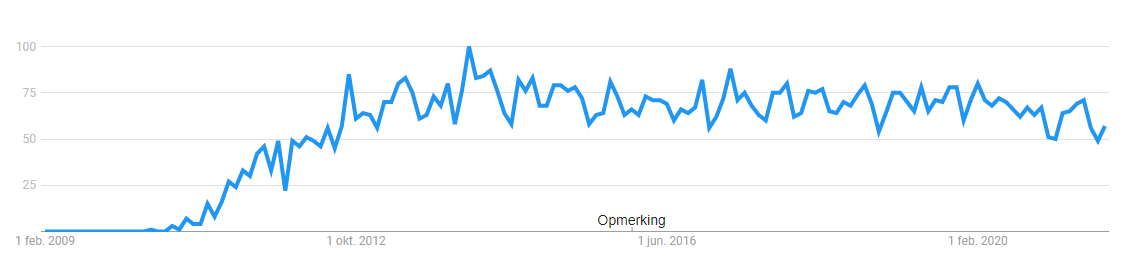
\includegraphics[width=\linewidth]{GoogleTrends.png}
    \caption{Populariteit van gamification \autocite{GoogleTrends2021}.}
    \label{fig:googletrends}
\end{figure}

Bunchball\footnote{https://www.biworldwide.com/gamification/bunchball-nitro/} wordt gezien als het bedrijf dat de gamification-industrie lanceerde. Hun product, Bunchball Nitro, was het eerste technologische platform dat gamemechanismen integreerde in digitale, niet-gaming ervaringen. Sindsdien zijn er tal van toepassingen ontwikkeld binnen verschillende domeinen zoals productiviteit, financiën, gezondheid, onderwijs, duurzaamheid, nieuws en entertainment media \autocite{Groh2012}.

\section{Definitie}

Gamification wordt gebruikt om twee verschillende soorten van ontwikkelingen te beschrijven, \textit{intentional gamification} en \textit{emergent gamification}.

\textit{Intentional gamification} of doelbewuste gamification is een eerste ontwikkeling die volgens \textcite{Deterding2011} wordt beschreven als het gebruik van elementen uit game-design in een niet-gaming context. Het is een opzettelijk proces waarbij een soortgelijke ervaring als in games wordt gecreëerd door activeiten, systemen, diensten of producten om te vormen of te verbeteren. Dit heeft als doel om veranderingen in het gedrag van de gebruiker teweeg te brengen.

\textit{Emergent gamification} of opkomende gamification is een tweede ontwikkeling die dan weer kan worden gedefinieerd als een opkomende, geleidelijke transformatie van cultuur en samenleving die het gevolg is van de steeds groeiende invloed van games. Er wordt verondersteld dat, door de steeds grotere rol van games in het leven van mensen, culturele en maatschappelijke praktijken geleidelijk veranderen in praktijken die kenmerkend zijn aan games, gaminggemeenschappen en spelerspraktijken  \autocite{Hamari2019}.

Zoals eerder werd vermeld, wordt gamification gedefinieerd als het gebruik van elementen uit game-design in een niet-gaming context. Mogelijke doelstellingen worden hierbij uitdrukkelijk weggelaten, dit om de definitie niet onnodig te gaan beperken. In plaats daarvan baseert het zich op de volgende semantische componenten: (1) \textit{game}, (2) \textit{elementen}, (3) \textit{ontwerp} en (4) \textit{niet-gaming context} \autocite{Sailer2016}.

\begin{enumerate}[label=(\arabic*)]
    \item Allereerst moet een onderscheid gemaakt worden tussen \textit{game} of spel en \textit{play} of spelen. Play wordt opgevat als een brede categorie die games omvat maar er van verschilt. \textcite{Caillois2001} verwijst naar het verschil tussen deze twee termen in zijn concept van \textit{paidia} en \textit{ludus}, twee polen van spelactiviteiten. \textit{Paidia} beschrijft vrije, expressieve, improviserende houdingen en betekenissen terwijl \textit{ludus} gekenmerkt is door op regels gebaseerde spellen met vastgelegde doelen. Gamification focust zich zo goed als exclusief op \textit{ludus} met slechts een kleine ruimte voor \textit{paidia}. Gamification heeft dus met andere woorden te maken met de op regels gebaseerde, doelgerichte aard van games \autocite{Sailer2016}.
    \item \textit{Elementen} laten toe om gamification te gaan onderscheiden van ``serieuze games''. In tegenstelling tot ``serieuze games'', omschreven als volwaardige games voor specifieke, niet-entertainment doeleinden, verwijst gamification naar het gebruik van verschillende bouwstenen van games die zijn geïntegreerd in reële contexten \autocite{Groh2012}. \textcite{Deterding20112} stellen voor om game-design elementen te gaan definiëren als elementen die kenmerkend zijn voor games, die voorkomen in de meeste (maar niet noodzakelijk alle) games en een belangrijke rol spelen in de werking en betekenis van de game.
    \item De term \textit{ontwerp} stelt game-design tegenover game-gebaseerde technologieën. De definitie van gamification heeft specifiek betrekking op een doelbewust ontwerpproces terwijl game-gebaseerde technologieën betrekking hebben op facetten zoals game-engines of controllers \autocite{Sailer2016}.
    \item Binnen de \textit{niet-gaming context} wordt er niet nader op ingegaan op de mogelijke gebieden waarin gamification kan worden toegepast, zodat de gebruikscontexten, -doeleinden of -scenario's niet worden afgebakend \autocite{Sailer2016}. De enige context die is uitgesloten, is gamification van games zelf. Dit omdat het een extensie zou zijn van een game zelf en dus als gevolg een deel is van game-design en niet van gamification \autocite{Groh2012}.
\end{enumerate}

\section{De vijf niveaus van game-design}

\textcite{Deterding20112} hebben in hun zoektocht doorheen de bestaande literatuur over games en gamification vijf game-design elementen geïdentificeerd bestaande uit verschillende abstractieniveaus. In Figuur \ref{fig:table1} worden ze gesorteerd op hun abstractieniveau, met bovenaan de meest concrete en onderaan de meeste abstracte.

\begin{figure}
    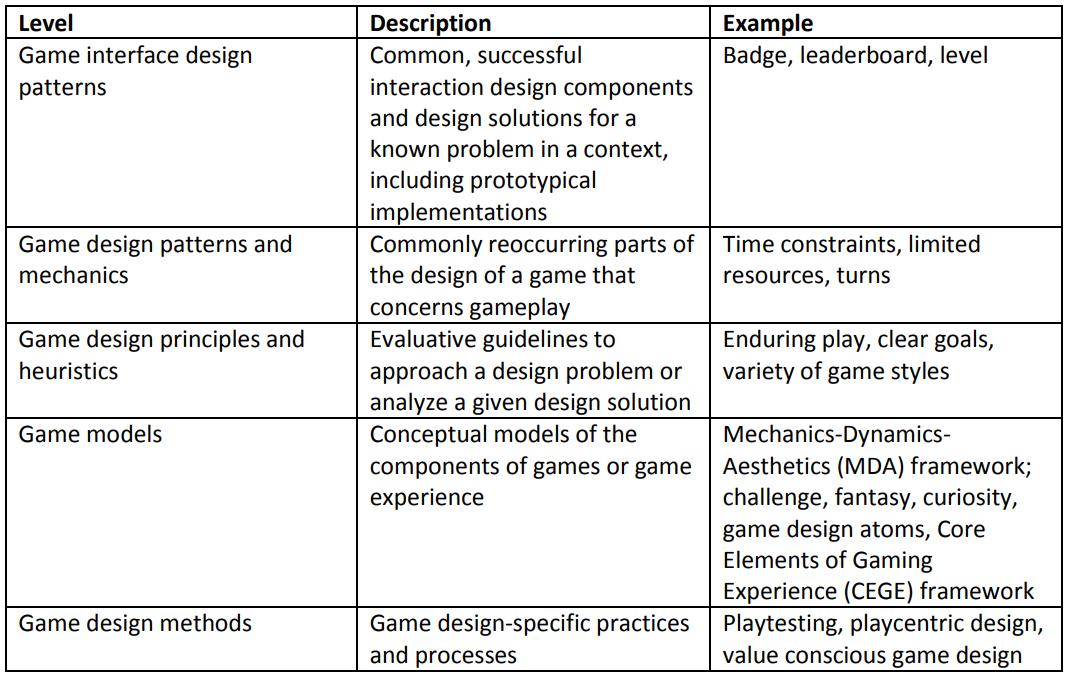
\includegraphics[width=\linewidth]{Deterding2011Table.png}
    \caption{Game-design elementen \autocite{Deterding20112}.}
    \label{fig:table1}
\end{figure}

\subsection{Game-interface ontwerppatronen}

De eerste categorie bevat veelvoorkomende, succesvolle interactie-ontwerpcomponenten, ontwerpoplossingen voor een gekend probleem binnen een bepaalde context en implementaties van prototypes. Badges, leaderboards en levels zijn een aantal voorbeelden van dit game-design element. Het zijn visuele indicatoren die prestaties van gebruikers weergeven \autocite{Morford2014}. Game-interface ontwerppatronen zijn dus met andere woorden elementen die betrekking hebben op wat er getoond gaat worden op het scherm van de gebruiker \autocite{Lindholm2016}.

\subsection{Game-designpatronen en -mechanismen}

Het tweede element wordt beschreven als vaak terugkerende onderdelen van het design van een game die te maken hebben met de gameplay. Deze onderdelen zijn iets wat gebruikers ervaren. Voorbeelden van deze game-designpatronen en -mechanismen zijn tijdsbeperkingen, beurten en beperkte middelen \autocite{Lindholm2016}. \textcite{Morford2014} beschrijven dit element als eigenschappen van een game waarmee gebruikers direct mee omgaan.

\subsection{Game-designprincipes en -heuristieken}

Het derde game-design element gaat over beoordelingsrichtlijnen om een ontwerpprobleem te gaan benaderen of een gegeven ontwerpoplossing te gaan analyseren. Langdurig spelen, duidelijke doelen en een verscheidenheid aan speelstijlen zijn een aantal voorbeelden die de game-designprincipes en -heuristieken karakteriseren.

\subsection{Gamemodellen}

Het vierde niveau heeft betrekking op conceptuele modellen van de componenten van games of game-evervaring. Een aantal van de voorbeelden die eigen zijn aan dit niveau zijn uitdaging, fantasie en nieuwsgierigheid. Het niveau van gamemodellen gaat met andere woorden over conceptuele benaderingen voor het begrijpen van de spelerservaring \autocite{Lindholm2016}.

\subsection{Game-designmethoden}

Ten slotte heeft het vijfde en laatste element te maken met specifieke game-design praktijken en processen ofwel game-design strategieën. Voorbeelden hiervan zijn playtesting, spelgericht ontwerpen en waardebewust game-design.

\section{Vaak voorkomende elementen}

Hieronder worden een aantal van de meest voorkomende en meest besproken game-design elementen meer in detail bekeken. Deze elementen worden nader bekeken door hun directe zichtbaarheid voor de spelers, doordat ze gemakkelijk geactiveerd of gedeactiveerd kunnen worden en omdat ze spelers sterk kunnen motiveren. Ze worden gemakkelijk geïmplementeerd door spelontwerpers omdat ze deel uitmaken van het zichtbare gedeelte van een game en niet van afhankelijk zijn van onderliggende mechanismen \autocite{Sailer2016}.

\subsection{Punten}

Punten zijn een van de elementen die aan de grondslag liggen van een groot aantal toepassingen die gamification implementeren en zijn hierdoor een basisvereiste \autocite{Sailer2016}. Ze zijn de gemakkelijkste manier om een speler te gaan belonen voor de succesvolle voltooiing van een actie, opdracht of een reeks van stappen en om hun vooruitgang in cijfervorm uit te drukken. Deze techniek is nuttig om mensen te gaan motiveren die graag een gevoel van vooruitgang hebben en om mensen aan te moedigen om acties te ondernemen \autocite{Costa2019}.

Voor de ontwerper zijn de punten ook belangrijk want ze houden de acties van alle spelers bij. Op deze manier kan gezien worden hoe spelers omgaan met het systeem, kan het systeem ontworpen worden voor bepaalde resultaten te behalen en kunnen de juiste aanpassingen aan het systeem gedaan worden \autocite{Zichermann2011}.

Het aantal punten dat wordt toegewezen aan een bepaalde actie moet zorgvuldig worden gekozen. Het is imperatief dat de punten afhankelijk zijn van de moeilijkheidsgraad van een taak of actie. Als een speler veel moeilijkheid ondervindt tijdens het uitvoeren van een taak en hiervoor minder punten krijgt zal hij/zij ontmoedigd geraken. Aan de andere kant, als een speler meer punten krijgt voor een makkelijke opdracht zal hij/zij gedemotiveerd geraken \autocite{Costa2019}.

\begin{figure}
    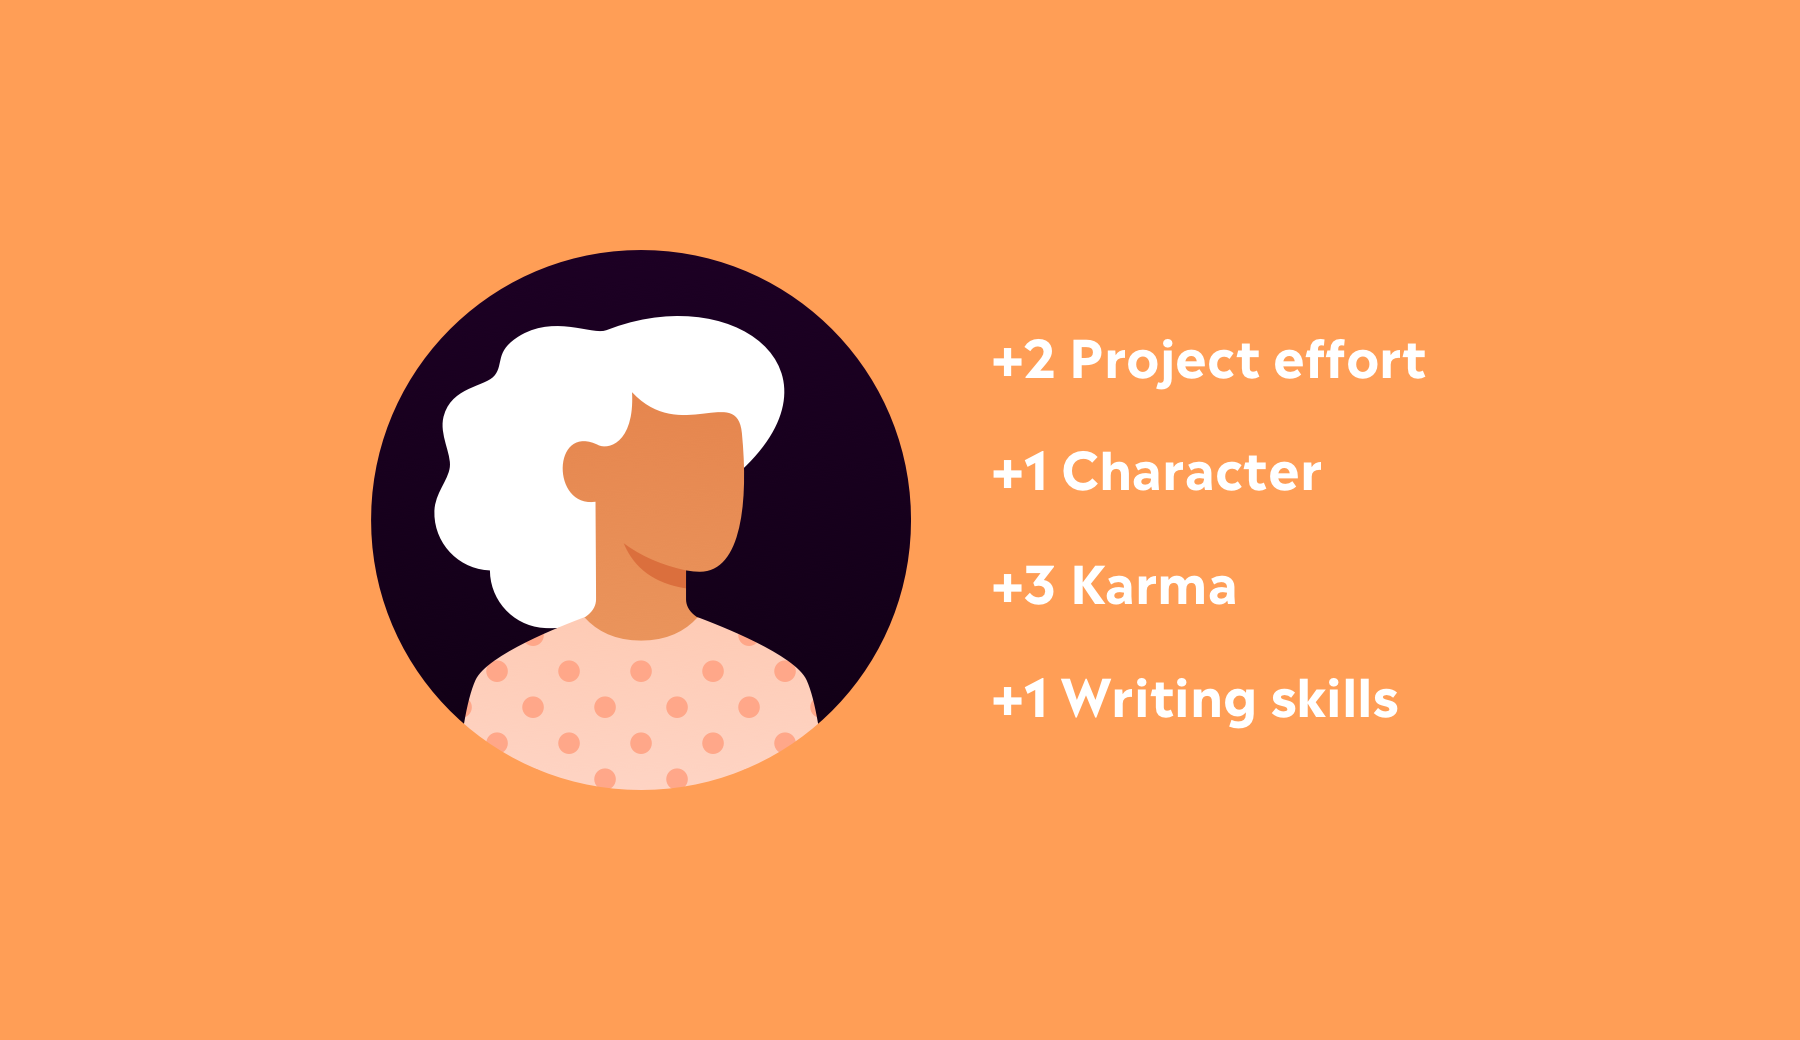
\includegraphics[width=\linewidth]{Points.png}
    \caption{Ervaringspunten \autocite{Points2018}.}
    \label{fig:points}
\end{figure}

Puntensystemen bestaan in alle soorten en maten, van overduidelijk tot nauwelijks zichtbaar \autocite{Zichermann2011}. Een aantal voorbeelden van deze systemen zijn ervaringspunten (weergegeven in Figuur \ref{fig:points}), inwisselbare punten of reputatiepunten \autocite{Sailer2016}. Ook kunnen de punten gerelateerd worden aan andere systemen, zoals leaderboards of niveaus \autocite{Costa2019}.

\subsection{Badges}

Badges worden gedefinieerd als een visuele voorstelling van prestaties of vaardigheden \autocite{Costa2019}. Ze kunnen zowel verdiend als verzameld worden. Het verdienen van een badge kan afhankelijk zijn van bijvoorbeeld een bepaald aantal punten te verzamelen of, zoals weergegeven in Figuur \ref{fig:badges}, een bepaalde activiteit uit te voeren \autocite{Sailer2016}.

\begin{figure}
    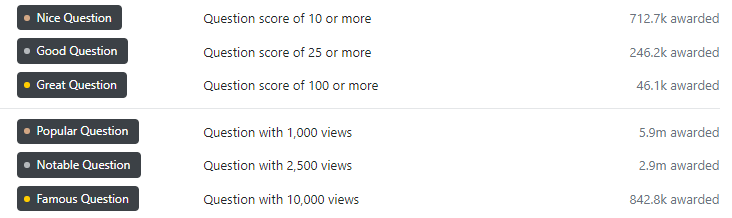
\includegraphics[width=\linewidth]{Badges.png}
    \caption{Badges met hun vereiste acties \autocite{Badges2021}.}
    \label{fig:badges}
\end{figure}

Een badge kan voorkomen in twee verschillende soorten, de zichtbare badges en onzichtbare badges. Een badge is zichtbaar als een speler weet welke actie hij/zij moet ondernemen of welk doel hij/zij moet bereiken. Een onzichtbare badge is een verrassing en wordt op een natuurlijke manier verdiend \autocite{Costa2019}.

Badges kunnen gebruikt worden als referentiesysteem dat de prestaties van spelers bevestigt, hun verdiensten symboliseert, zichtbaar aantoont dat spelers een niveau of doel hebben bereikt \autocite{Anderson2013} en de voortgang van het spel binnen het systeem weergeeft \autocite{Zichermann2011}. Ook kunnen ze fungeren als stimulans, doordat een gebruiker bepaalde acties zal ondernemen om een badge te behalen. Hierdoor wordt het gedrag van gebruikers in een gewenste richting gestuurd. Ten slotte kunnen badges ook dienen als statussymbool, vooral als ze zeldzaam zijn of moeilijk te verdienen \autocite{Sailer2016}. Dit kan opnieuw spelers beïnvloeden om dezelfde acties of stappen te ondernemen om dezelfde badges te verdienen.

\subsection{Scoreborden}

Scoreborden geven een overzicht van deelnemers aan een competitie \autocite{Costa2013} en rangschikken hen volgens hun relatieve succes. Standaard wordt een geordende lijst weergegeven met een score naast elke naam \autocite{Zichermann2011}. Deze score wordt bepaald aan de hand van een succescriterium \autocite{Sailer2016}. Dit succescriterium kan bijvoorbeeld het aantal verzamelde punten zijn.

Een scorebord helpt om te bepalen wie het beste presteert door de prestaties van spelers voor anderen zichtbaar te maken \autocite{Costa2019}. Doordat spelers een eenvoudige vergelijking kunnen maken tussen hun eigen prestaties en die van anderen \autocite{Zichermann2011} kan de competitie tussen spelers in stand gehouden worden. Als dit in de juiste situatie wordt gebruikt kan een scorebord een krachtige motivator zijn \autocite{Costa2019}. Echter kunnen ze ook fungeren als demotivator als spelers zich aan de onderkant van het leaderboard bevinden \autocite{Sailer2016}.

\begin{figure}
    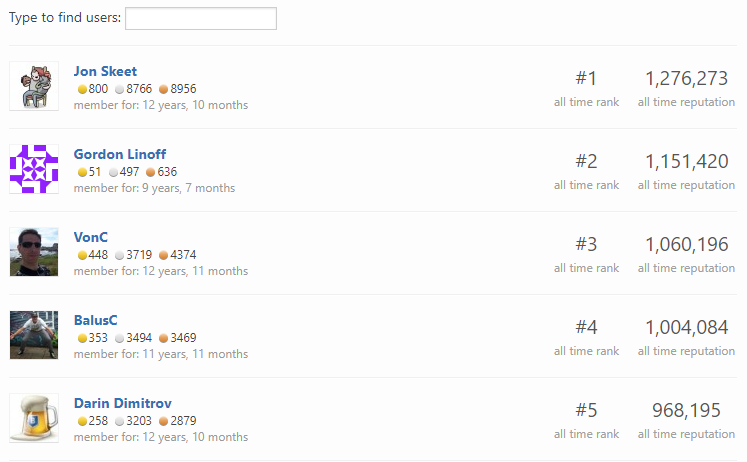
\includegraphics[width=\linewidth]{Leaderboard.png}
    \caption{Reputatiepunten van de top vijf gebruikers \autocite{Leaderboard2021}.}
    \label{fig:leaderboard}
\end{figure}

Er zijn verschillende manieren om een scorebord te ontwerpen. Een ontwerper kan ervoor kiezen om slechts een bepaald deel weer te geven, om geen competitief gedrag aan te moedigen. Dit kan bijvoorbeeld door slechts twee personen boven en onder een speler weer te geven, om hij/zij aan te motiveren. Zoals in Figuur \ref{fig:leaderboard} wordt getoond, kan de ontwerper beslissen om de competitie te vergroten door enkel de top vijf van alle spelers te tonen, waardoor spelers worden aangemoedigd hun score te vergroten \autocite{Costa2019}.

\subsection{Prestatiegrafieken}

Prestatiegrafieken geven informatie weer over de prestaties van een speler in vergelijking met zijn/haar eerdere prestaties \autocite{Sailer2013}. Ze geven dus in tegenstelling tot scoreborden, waar de prestaties van een speler worden vergeleken met die van andere spelers, een evaluatie van de verwezenlijkingen van een speler over een bepaalde periode \autocite{Sailer2016}.
 
Door de prestaties grafisch weer te geven over een bepaalde periode krijgt de speler feedback over zijn/haar verwezenlijkingen, waardoor wordt aangemoedigd om de focus te leggen op verbetering \autocite{Sailer2013}.

\subsection{Betekenisvolle verhalen}

Een betekenisvol verhaal is een ontwerpelement dat niet direct gerelateerd is aan de prestaties van een speler \autocite{Sailer2016}. Binnen platformen die gamification implementeren kunnen, door het toevoegen van een verhaal, activiteiten en opdrachten binnen een bepaalde context worden geplaatst. Ze krijgen hierdoor een betekenis die verder gaat dan louter een zoektocht naar punten en prestaties \autocite{Kapp2012}.

Door een betekenis te geven aan activiteiten en opdrachten krijgen spelers een gevoel van inspiratie en motivatie, vooral als het verhaal aansluit bij hun persoonlijke interesses \autocite{Sailer2016}. Verhalen kunnen ook positieve gevoelens opwekken en versterken \autocite{Sailer2013}.

\subsection{Avatars}

Avatars zijn een visuele representatie van de speler binnen de gamification omgeving \autocite{Sailer2016}. De avatar wordt meestal zelf gekozen of gecreërd \autocite{Kapp2012}. Ze delen de identiteit, aanwezigheid, locatie, en activiteiten van de speler met anderen \autocite{Annetta2010}.

Een avatar kan een een complexe, geanimeerde driedimensionale representatie zijn \autocite{Sailer2016} maar kan ook eenvoudigweg een kleine pictogram zijn met een gebruikersnaam \autocite{Zichermann2011}. De belangrijkste vereiste is dat ze de spelers identificeren en hen onderscheiden van anderen \autocite{Sailer2016}.

Gelijk welke vorm een avatar aanneemt, ze laten toe dat de speler een andere identiteit kan aannemen en deel kan uitmaken van een gemeenschap \autocite{Annetta2010}. Dit kan spelers een gevoel van autonomie geven en positieve gevoelens geven door een ontwikkelingsproces met de avatar aan te gaan \autocite{Sailer2013}.

\subsection{Teamleden}

Door teams te introduceren, gedefinieerd als afgebakende groepen van spelers die samenwerken aan een doel, kan samenwerking worden bevorderd \autocite{Sailer2016}. Tussen de verschillende teamleden kan echter ook een rivaliteit tot stand komen of kunnen conflicten ontstaan \autocite{Kapp2012}.

\section{Gedrag beïnvloeden}

Een van de belangrijkste doelen van gamification is het gedrag van een gebruiker beïnvloeden \autocite{AlMarshedi2015}. Volgens het gedragsmodel van \textcite{Fogg2009} moet een persoon of gebruiker eerst een bepaald niveau van motivatie bereiken en de mogelijkheid krijgen om het gedrag te vertonen. Zodra deze twee toestanden zijn bereikt is enkel nog een trigger nodig om het gewenste gedrag tevoorschijn te laten komen.

\subsection{Motivatie}

Motivatie is het verlangen om iets te doen. Het is belangrijk om hiermee rekening te houden bij gamification, in het bijzonder omdat het gedrag van mensen stuurt \autocite{AlMarshedi2015}. In het algemeen bestaan twee soorten van menselijk motivatie: (1) \textit{intrinsieke motivatie} en (2) \textit{extrinsieke motivatie} \autocite{Yang2017}.

\begin{enumerate}[label=(\arabic*)]
    \item \textit{Intrinsieke motivatie} wordt gedefinieerd als een intern verlangen om dingen te doen uit plezier of liefde \autocite{AlMarshedi2015}, ofwel een activiteit nastreven omdat deze inherent interessant of plezierig is. Wanneer een persoon intrinsiek gemotiveerd is, zal hij/zij dus bewogen worden om te handelen voor het plezier of de uitdaging in plaats van te bewogen te worden vanwege beloningen of externe druk. Het is een natuurlijke aanleg voor ontdekking, bekwaamheid en spontane interesse dat de volharding, prestaties en het welzijn ten goede komen \autocite{Dahlstrom2018}. 
    \item \textit{Extrinsieke motivatie} kan worden beschreven als dingen doen uitsluitend voor het resultaat \autocite{AlMarshedi2015}. Het wordt vaak geassocieerd met voornamelijk de wens om beloningen te krijgen en bestraffing te vermijden, wat wordt gezien als minder ideaal voor het welzijn van mensen dan intrinsieke motivatie. Extrinsieke motivatie kan sterk variëren in welke vorm deze voorkomt en kan toch leiden tot een grotere ervaring van welzijn, afhankelijk  van hoeveel gevoel van autonomie deze de persoon in kwestie geeft \autocite{Dahlstrom2018}.
\end{enumerate}

Een groot aantal gamificationtoepassingen en -diensten richten zich tegenwoordig op motivatie, vooral van het extrinsieke type. Extrinsieke motivatie kan echter niet als enige manier gebruikt worden om gedrag te veranderen. Dit komt omdat extrinsieke motivatie sterk afhangt van individuele kenmerken. De gedragsverandering kan dus van tijdelijke aard zijn en zorgt dus niet voor een duurzaam effect. Een goed inzicht krijgen in de verschillende soorten van motivatie en hoe gedrag tot stand komt is dus van cruciaal belang bij het ontwerpen van toepassingen en diensten die gamification implementeren \autocite{AlMarshedi2015}.

\section{Hexad Framework}

De ``Big Five'' persoonlijkheidsfactoren, een beschrijvend model van persoonlijkheid, is in het verleden al uitgebreid gebruikt geweest om de psychologie achter gebruikersmotivatie te onderzoeken \autocite{Yuan2016}. Dit model schiet echter tekort omdat het niet specifiek bedoeld is voor gamification.

Om een beter inzicht te krijgen in wat de gebruiker motiveert en om de ervaring te personaliseren binnen een omgeving die gamification implementeerd, hebben \textcite{Tondello2016} het Hexad Framework ontwikkeld. Het is specifiek ontworpen naar gebruikersmotivatie binnen gamification en het dient om zes gebruikerstypes te linken aan verschillende ontwerpelementen.

\subsection{Gebruikerstypes}

\textcite{Marczewski2015} stelde zes gebruikerstypes voor, zichtbaar in Figuur \ref{fig:usertypes}, die verschillen in de mate waarin ze gemotiveerd kunnen worden door intrinsieke of extrinsieke motiverende factoren, namelijk (1) \textit{filantropen}, (2) \textit{socialisers}, (3) \textit{vrije geesten}, (4) \textit{presteerders}, (5) \textit{spelers} en (6) \textit{ontwrichters}.

\begin{enumerate}[label=(\arabic*)]
    \item \textit{Filantropen} zijn altruïstisch en zijn bereid om te geven zonder een beloning te verwachten. Ze worden gemotiveerd door een doel. Enkele van de voorgestelde ontwerpelementen voor filantropen zijn: verzamelen en handelen, schenken, delen van kennis en administratieve rollen.
    \item \textit{Socialisers} willen met anderen omgaan en social banden scheppen. Ze worden gemotiveerd door verwantschap. Ontwerpelementen die socialisers motiveren zijn teams, sociale netwerken, social vergelijking, sociale competitie en sociale ontdekking.
    \item \textit{Vrije geesten} worden gemotiveerd door autonomie, meer bepaald vrijheid om zichzelf te uiten en te handelen zonder controle van buitenaf. Ze willen vooral creëren en verkennen binnen een systeem. De ontwerpelementen die het beste bij hun passen zijn: verkennende taken, tools voor creativiteit, ontgrendelbare content, niet-lineaire gameplay en Easter eggs.
    \item Competentie is de sterkste motivator voor \textit{presteerders}. Ze proberen vooruit te geraken binnen een systeem door taken te voltooien of moeilijke uitdagingen aan te gaan. Uitdagingen, certificaten, het leren van nieuwe vaardigheden, niveaus en progressie zijn enkele van de elementen die bij hun passen.
    \item \textit{Spelers} zullen er alles aan doen om een beloning te verdienen binnen een systeem, ongeacht het type activiteit. Ze worden het meeste gemotiveerd door extrinsieke beloningen. Ontwerpelementen waarvoor spelers de voorkeur hebben zijn punten, scoreborden, badges, beloningen of prijzen en virtuele economieën.
    \item \textit{Ontwrichters} willen verandering teweegbrengen. Ze willen het systeem ontwrichten, op zowel een positieve als negatieve manier, om veranderingen af te dwingen. Ze houden ervan om de grenzen van het systeem af te tasten en deze grenzen steeds verder te verleggen. Enkele voorgestelde ontwerpelementen zijn: innovatieplatformen, ontwerptools, anonimiteit en anarchistische gameplay.
\end{enumerate}

Het is belangrijk om op te merken dat individuen zelden binnen één bepaald type passen. Gebruikers zullen vaak een hoofdtendens vertonen maar ze zullen in de meeste gevallen ook tot op zekere hoogte binnen andere types passen \autocite{Tondello2016}.

\begin{figure}
    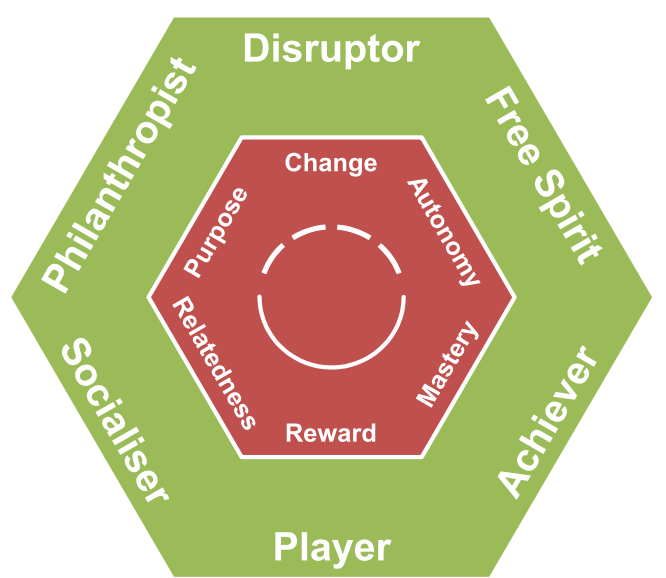
\includegraphics[width=\linewidth]{HexadUserTypes.png}
    \caption{De Hexad gebruikerstypes \autocite{Tondello2016}.}
    \label{fig:usertypes}
\end{figure}

\subsection{Methodologie}



Via de voorgestelde enquête en data-analyse kunnen ontwerpers hun doelpubliek screenen en de juiste ontwerpelementen kiezen, gepersonaliseerd voor elke gebruiker. Binnen onderzoek kunnen de resultaten gebruikt worden om een beter begrip te krijgen over de betrokkenheid van gebruikers en hun plezier van gebruik \autocite{Tondello2016}.


